
\subsection{Testing the Effective Correlation Space}
\label{sxn:empirical-effective_corr_space}

Here, we will address the question: 
\begin{quote}
How shall we \emph{test the assumption} of the \EffectiveCorrelationSpace?
\end{quote}
Recall that the \SETOL theory estimates model quality by evaluating the ST \GeneralizationError as an integral over the theoretical training data $\boldsymbol{\xi}$.
This integral assumes each layer weight matrix can be replaced with an effectively lower rank form, i.e., $\mathbf{W}\rightarrow\mathbf{W}^{\EFF}$, corresponding to the span of the eigencomponents defined by the tail of the ESD, $\rho_{tail}(\lambda)$. 
In the \HTSR \Phenomenology, the tail is defined by the fact that $\rho_{tail}(\lambda)$ follows a PL distribution, above some minimal value $\lambda_{min}$.
In our \SETOL theory, the tail is defined by choosing the minimal value $\lambda_{min}$ to satisfy the Empirical Trace-Log condition.
%
These methods of realizing $\mathbf{W}^{\EFF}$ are essentially \emph{Model Selection Rules} (MSRs) for the \EffectiveCorrelationSpace. 
%By ``\ModelSelectionRule, we refer to a procedure to choose a $\lambda_{min}$ such that all eigenvalues above $\lambda_{min}$ are included in the tail. 
%
Importantly, in neither approach is $\lambda_{min}$ just some ``rank parameter to be chosen by yet some other MSR on 
the basis of rank, or magnitude alone, (that, in particular, does not know about \HTSR or \SETOL, which consider the 
\emph{shape} of the ESD).

Thus, to test the assumption of the \EffectiveCorrelationSpace, we want to show that the models predictions are in fact controlled predominantly by the tail, where the specific choice of the rank parameter depends on \HTSR or \SETOL as we expect.
We can emulate this theoretical construct and estimate (trends in the) test accuracies by evaluating the train and/or 
test accuracies of the trained MLP3 model -- after replacing the MLP3 layer weight matrices $\mathbf{W}_{FC1}$ and $\mathbf{W}_{FC2}$ with a low-rank approximation consisting of \emph{only} the tail:
% using a TruncatedSVD method:
\begin{align*}
 \mathbf{W}^{\EFF}_{FC1}:= P_{tail}\mathbf{W}_{FC1} \\
 \mathbf{W}^{\EFF}_{FC2}:= P_{tail}\mathbf{W}_{FC2}  ,
\end{align*}
where $P_{tail}$ is a projection operator selecting only the tail of the ESD with TrucnatedSVD.
(That is, we will use the  low-rank TruncatedSVD approximation at the inference step, not at the training step, as is more common.)
A Truncated model is one whose weight matrices $\mathbf{W}_*$ have been replaced by truncated matrices $\mathbf{W}^{\EFF}_*$. 
We denote the difference between the original models accuracy and the Truncated models train and test accuracy as $\Delta E_{train}$ and $\Delta E_{test}$, respectively:
\begin{align*}
  \Delta E_{train}:=  E_{train}(\mathcal{D}) - E^{\EFF}_{train}(\mathcal{D}) \\
  \Delta E_{test}:=  E_{test}(\mathcal{D}) - E^{\EFF}_{test}(\mathcal{D})  ,
\end{align*}
where $E^{\EFF}_{train}$ denotes the error of the TruncatedSVD model on the training portion of the dataset $\mathcal{D}$,a
and  $E^{\EFF}_{test}$ denotes corresponding test error for the TruncatedSVD model.
%$\Delta E$ denotes the difference between test and/or training accuracies (for difference batch sizes $bs$).

\paragraph{The \POWERLAW~and \TRACELOG~Model Selection Rules}
\charles{is MSR still a good theme here?  In the orginal paper we discussed the MSR up front. Now
  we seem to just casually mention it here.}
If we use good MSRs, then we expect that $\Delta E_{train}\to 0$ and $\Delta E_{test}\to 0$ as the models approach \IdealLearning. 
%
We consider the following MSRs,%
\footnote{We considered other MSRs that do not ``know about \HTSR or \SETOL, but they (expectedly) perform in trivial or uninteresting ways for testing the assumption of the \EffectiveCorrelationSpace.  Thus, we are not introducing just some arbitrary low-rank approximation, as is common, but instead that the specific \SETOL-based MSR matters.} 
which are associated with the \HTSR and \SETOL approaches.
\begin{itemize}
\item 
The \POWERLAW~MSR: 
All eigenvalues lying in the tail of the ESD, 
$\lambda_i \ge \LAMBDAPL$, where $\LAMBDAPL$ is the start of the PL tail, as determined by the \WW~PL fit, which is based on \cite{CSN09_powerlaw}.
\item 
The \TRACELOG~MSR: 
All eigenvalues lying in the tail of the ESD, 
such that they satisfy the Trace-Log Condition, i.e., $\lambda_{i}\ge \LAMBDADETX$, where $\prod\lambda_{i:\lambda_i \ge \LAMBDADETX}\simeq 1$.
\end{itemize}
\chris{CH TODO: Find a place to call out the need for Normalizing $W$ to Frobenius norm = $M$.}


%\chris{I commented out the part about Kendals tau rank statistics. Lets discuss if we would like to add it back in}
%The MSRs lead directly to data-dependent quality metrics. By this, 
%we mean metrics that directly evaluate the train error of the model,
%using the actual training data $\mathcal{D}$, and with either the unmodified (i.e. bare)
%or some modified (i.e effective, smoothed)  model.  
%
%Then, we can compare and contrast the different MSRs in order to
%see how well they can predict the trends in the test accuracies
%for the different batch sizes.
%We do this visually and by computing the rank correlation 
%between the actual $E_{test}$ and predicted $E^{\EFF}_{train}(\mathcal{D})$
%(i.e. with the Kendall-tau rank correlation metric).

%\item The \SVDA~and \SVDB MSRs:  The \SVDA retains the top $20\%$ of the eigenvalues of the tail of the ESD, and the \SVDB~MSR retains the  top $40\%$.
%For all MSRs, we apply the TruncatedSVD approximation to $\mathbf{W}$, keeping only those
%eigencomponenents associated with the eigenvalues in the tail. 


%\chris{There are 6 plots for each MSR, but I think showing 3 gets the point across. Just remove comments below to add 
%them back in.}


\subsubsection{Train and test errors by epochs}
\label{sxn:trunc_err_epochs}
\begin{figure}[t]
    \centering
    \subfigure[$lr=1\times$]{
        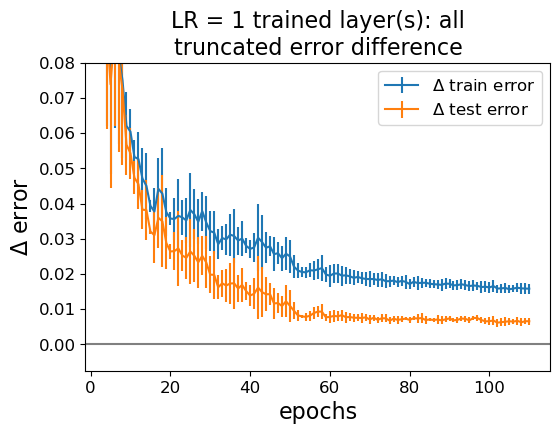
\includegraphics[width=4cm]{img/truncated_error/mlp3_trunc_error_by_epochs_LR_0_all_xmin.png}
        \label{fig:mlp3-trunc_err_epochs_xmin_1}
    }
    \subfigure[$lr=2\times$]{
        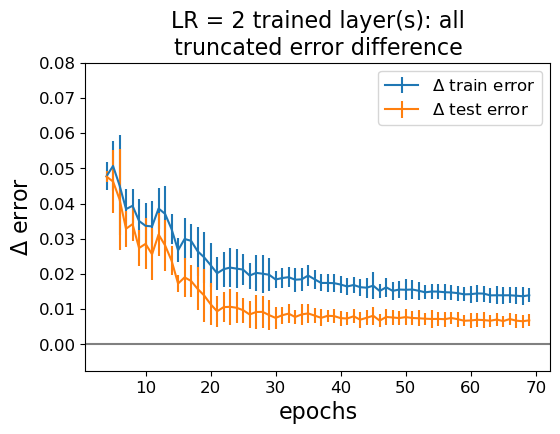
\includegraphics[width=4cm]{img/truncated_error/mlp3_trunc_error_by_epochs_LR_1_all_xmin.png}
        \label{fig:mlp3-trunc_err_epochs_xmin_2}
    }
    \subfigure[$lr=4\times$]{
        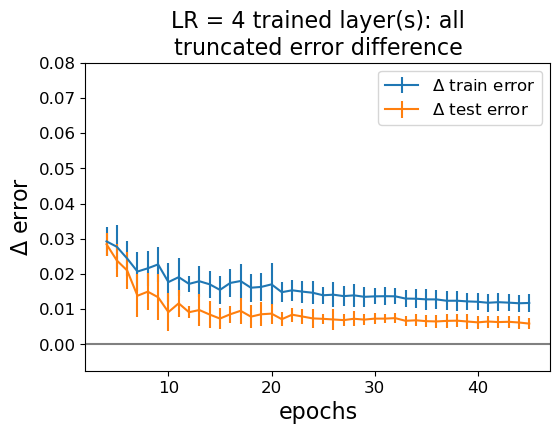
\includegraphics[width=4cm]{img/truncated_error/mlp3_trunc_error_by_epochs_LR_2_all_xmin.png}
        \label{fig:mlp3-trunc_err_epochs_xmin_4}
    }\\
    \subfigure[$lr=8\times$]{
        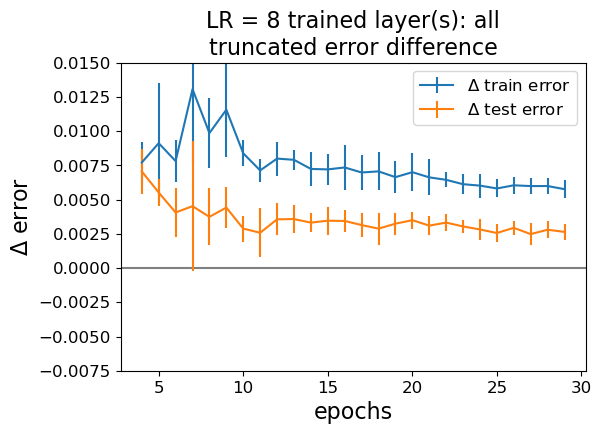
\includegraphics[width=4cm]{img/truncated_error/mlp3_trunc_error_by_epochs_LR_3_all_xmin.png}
        \label{fig:mlp3-trunc_err_epochs_xmin_8}
    }
    \subfigure[$lr=16\times$]{
        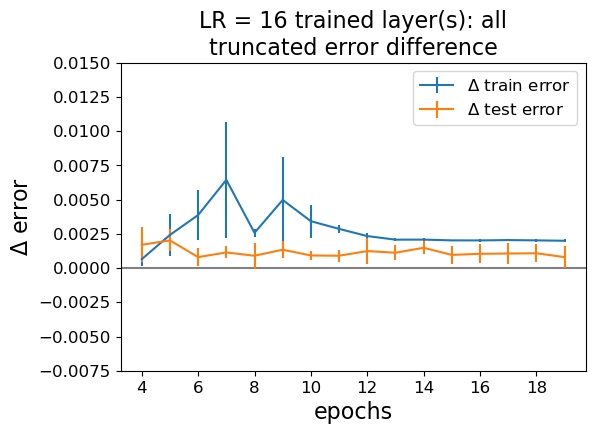
\includegraphics[width=4cm]{img/truncated_error/mlp3_trunc_error_by_epochs_LR_4_all_xmin.png}
        \label{fig:mlp3-trunc_err_epochs_xmin_16}
    }
    \subfigure[$lr=32\times$]{
        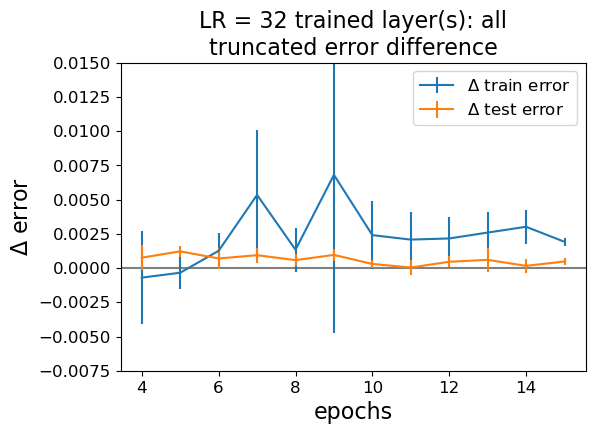
\includegraphics[width=4cm]{img/truncated_error/mlp3_trunc_error_by_epochs_LR_5_all_xmin.png}
        \label{fig:mlp3-trunc_err_epochs_xmin_32}
    }
    \caption{
            $\Delta E_{train}$ (blue) and $\Delta E_{test}$ (orange) for various learning rates, using the 
            \POWERLAW~MSR. As learning rate increases we can see that $\Delta E_{train}$ and $\Delta E_{test}$ both tend 
            towards lower asymptotic minima, which they reach after fewer epochs of training. We can also see that 
            (after the first few epochs,) $\Delta E_{train}$ (blue) is always higher than $\Delta E_{test}$ (orange). 
            Observe that in the bottom row (d--f) the yaxis is contracted to make the variation more visible. In (f) we can see 
            that as learning rate surpasses its optimal setting, the gap between $\Delta E_{train}$ and $\Delta 
            E_{test}$ begins to increase again, and has wider error bars, suggesting that the excessively large learning 
            rate is disrupting the MLP3s ability to lear the \EffectiveCorrelationSpace.
    }
    \label{fig:mlp3-msr-results-xmin}
    %Comparison of \POWERLAW~and \TRACELOG~ Model Selection Rules for testing the \EffectiveCorrelationSpace}
\end{figure}



To see how the \EffectiveCorrelationSpace forms, we plot how $\Delta E_{train}$ and $\Delta E_{test}$ evolve over training, for each of the various learning rates considered.%
\footnote{When batch size was varied, results did not significantly differ, and so they are omitted. 
%% CONFIRM WE HAVE SAID THIS ELSEWHERE %% See the experimental Colab notebooks for the full set of experiments.
} 

We start with the effect of the \POWERLAW~MSR.
See Figure~\ref{fig:mlp3-msr-results-xmin}, where we see that $\Delta E_{train}$ and $\Delta E_{test}$ generally trend 
downwards as they approach minimum train error. 
When the learning rate is larger, the models converge more quickly, and $\Delta E_{train}$ and $\Delta E_{test}$ also converge to lower values. 
Recall from Figure~\ref{fig:mlp3-accuracies-lr} that $lr=16\times$ had the lowest test error. In 
Figure~\ref{fig:mlp3-trunc_err_epochs_xmin_16}, we see that it also has the lowest $\Delta E_{train}$ and $\Delta 
E_{test}$. A lower $\Delta E_{train}$ or $\Delta E_{test}$ means that more of the models correct predictions are due to 
the low rank tail, meaning that the tail generalizes better, and we see here that when the tail generalizes best, the 
model was the most accurate. 

In each plot, we also see that the error bars are wide early on, before suddenly becoming much narrower. This transition 
is more visible in the larger learning rates shown in~\ref{fig:mlp3-trunc_err_epochs_xmin_8}--\ref{fig:mlp3-trunc_err_epochs_xmin_32},
but can also be seen in \ref{fig:mlp3-trunc_err_epochs_xmin_1}--\ref{fig:mlp3-trunc_err_epochs_xmin_4}, albeit less 
clearly. Most interestingly of all, this transition is preceded by a brief period, sometimes a single epoch, in which the 
error bars are drastically wider, in a way that is reminiscent of a first-order phase transition. Again, this 
phenomenon can be seen most clearly in ~\ref{fig:mlp3-trunc_err_epochs_xmin_8}--\ref{fig:mlp3-trunc_err_epochs_xmin_32}.


We next consider the effect of the \TRACELOG~MSR.
See Figure~\ref{fig:mlp3-msr-results-detX}, which also shows the development of $\Delta E_{train}$ and $\Delta E_{test}$ 
over epochs, where we see a very different pattern in the train error and test error. 
The difference in the train error is because, as the model is untrained in the early epochs, the \TRACELOG~MSR 
\emph{over}-estimates the tail by choosing a $\lambda_{min}$ that is too small. 
Thus, $\Delta E_{train}$ actually increases to its asymptotic value at the final epoch. 
In the earliest epochs, the truncated train error is even \emph{less} than the full MLP3 models error, suggesting that 
signal is forming in the large eigenvalues in these early epochs, but is swamped by the randomness of the early initial 
weights, some of which is then removed by truncation. As epochs progress, this effect disappears.
%
Here again we can see the ``phase-transition-like behavior of the train error, as the error bars are wide early on, up to a transition having an abnormally large error bar, after which they stabilize.

% \michael{@chris: we should have a few sentences on why the Delta-Error-Test is so flat.}
Perhaps most interestingly of all, we see that under the \TRACELOG~MSR, $\Delta E_{test}$ is flat \emph{throughout 
training}, and for all learning rates. Considering that this implies that there is \emph{no} point in training where the 
\TRACELOG tail generalizes badly, this is a rather striking observation. It also bears noticing that under the 
\POWERLAW~MSR, (Figure~\ref{fig:mlp3-msr-results-xmin},) this is decidedly not the case, meaning that a small, but 
significant amount of generalization comes from the gap between these tails, but none at all comes from the bulk.
\nred{confusing}


\begin{figure}[t]
    \centering
    \subfigure[$lr=1\times$]{
        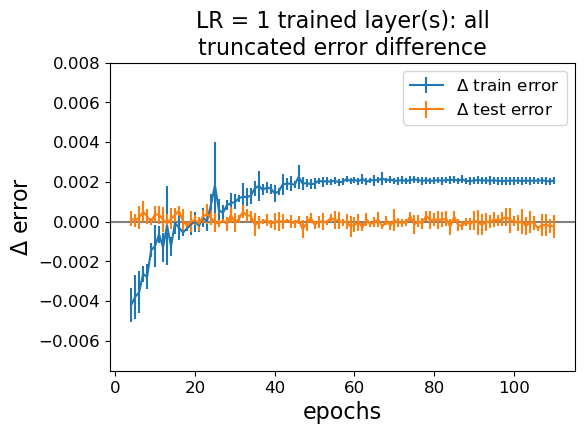
\includegraphics[width=4cm]{img/truncated_error/mlp3_trunc_error_by_epochs_LR_0_all_detX.png}
        \label{fig:mlp3-trunc_err_epochs_detX_1}
    }
    \subfigure[$lr=2\times$]{
        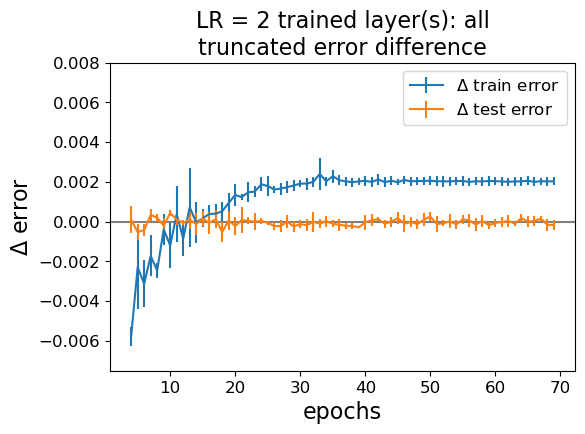
\includegraphics[width=4cm]{img/truncated_error/mlp3_trunc_error_by_epochs_LR_1_all_detX.png}
        \label{fig:mlp3-trunc_err_epochs_detX_2}
    }
    \subfigure[$lr=4\times$]{
        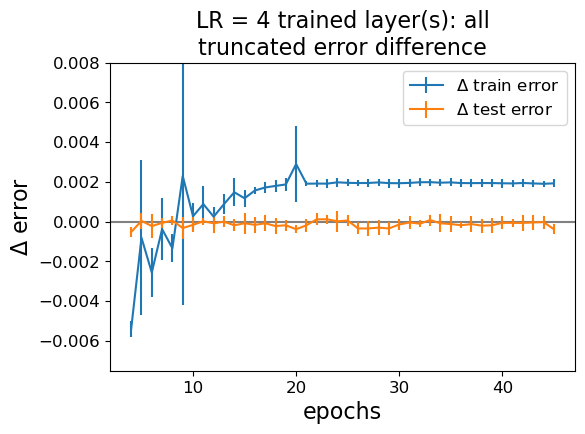
\includegraphics[width=4cm]{img/truncated_error/mlp3_trunc_error_by_epochs_LR_2_all_detX.png}
        \label{fig:mlp3-trunc_err_epochs_detX_4}
    }\\
    \subfigure[$lr=8\times$]{
        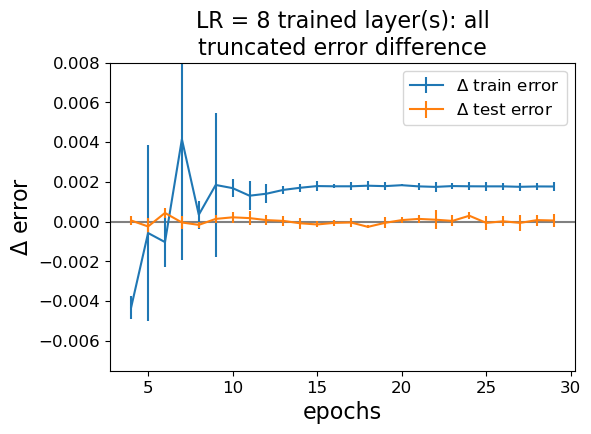
\includegraphics[width=4cm]{img/truncated_error/mlp3_trunc_error_by_epochs_LR_3_all_detX.png}
        \label{fig:mlp3-trunc_err_epochs_detX_8}
    }
    \subfigure[$lr=16\times$]{
        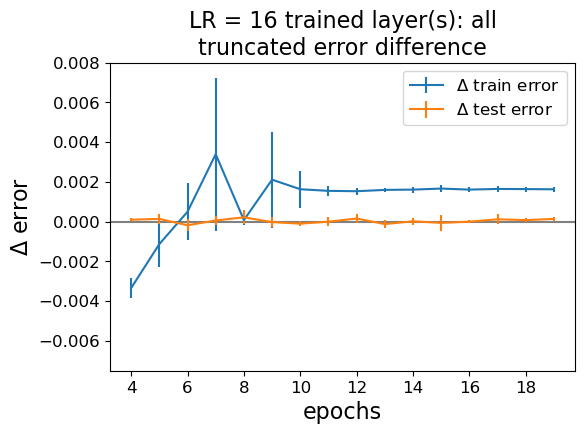
\includegraphics[width=4cm]{img/truncated_error/mlp3_trunc_error_by_epochs_LR_4_all_detX.png}
        \label{fig:mlp3-trunc_err_epochs_detX_16}
    }
    \subfigure[$lr=32\times$]{
        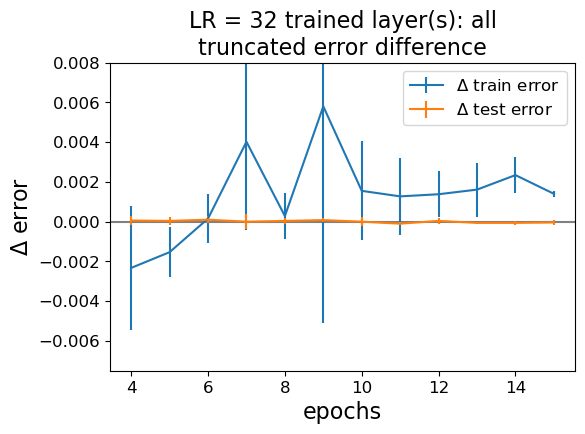
\includegraphics[width=4cm]{img/truncated_error/mlp3_trunc_error_by_epochs_LR_5_all_detX.png}
        \label{fig:mlp3-trunc_err_epochs_detX_32}
    }
    \caption{
        $\Delta E_{train}$ (blue) and $\Delta E_{test}$ (orange) for selected learning rates, using the \TRACELOG~MSR. 
        For all learning rates, $\Delta E_{test}$ is centered on $0$, meaning that the \TRACELOG~Effective Correlation 
        Space explains almost all variation in out-of-sample predictions, but it does \emph{not} explain all of the 
        training set predictions (blue). NOTE: The y axis is the same in all plots, and is much narrower than in 
        Figure~\ref{fig:mlp3-msr-results-xmin}. In (a--e) we can see that $\Delta E_{train}$ converges to approximately 
        $0.002$. Compare with Figure~\ref{fig:mlp3-trunc_err_epochs_xmin_16}, which reaches a minimum of approximately 
        $0.0025$. As in Figure~\ref{fig:mlp3-trunc_err_epochs_xmin_32}, the learning rate of $32\times$ normal disrputs the 
        MLP3s ability to discover the \TRACELOG \EffectiveCorrelationSpace.
    }
    \label{fig:mlp3-msr-results-detX}
    %Comparison of \POWERLAW~and \TRACELOG~ Model Selection Rules for testing the \EffectiveCorrelationSpace}
\end{figure}


There are two final points of comparison between Figures~\ref{fig:mlp3-msr-results-xmin} and~\ref{fig:mlp3-msr-results-detX}.
%
First, 
although it appears in Figure~\ref{fig:mlp3-msr-results-detX} that $\Delta E_{train}$ converges to a larger value than in Figure~\ref{fig:mlp3-msr-results-xmin}, this is because the scale of the y-axis is $10\times$ smaller. 
That is, the \POWERLAW~MSR is biased towards over-estimating $\lambda_{min}$, which means it over-truncates, producing a 
larger $\Delta E_{train}$ or $\Delta E_{test}$ 
than the \TRACELOG~MSR, which is biased towards under-estimating $\lambda_{min}$. 
%
Second,
in both Figure~\ref{fig:mlp3-msr-results-xmin} and~\ref{fig:mlp3-msr-results-detX}, we can see that $\Delta E_{test}$ is consisitently lower than $\Delta E_{train}$. 
Clearly, truncating has a larger effect on train predictions, meaning that no matter how long the model is trained, some 
of the train predictions are still derived from the bulk. 
Yet, the test predictions are far less affected, meaning that the \EffectiveCorrelationSpace contributes to the models ability to generalize.
% \michael{I as assuming that fig refers to Fig \ref{fig:mlp3-msr-results-detX} and not to Fig \ref{fig:mlp3-msr-results-xmin}? If, flesh out and put in the previous par.
% }
% \chris{Lets discuss. Im not sure what youre referring to here.}



%%We have shown that both MSRs can preserve and explain the test predictions on a simple model like MLP3
%%when the weight matrix is HT, but not necessarily when it is HT element-wise, (i.e has a \CorrelationTrap).
%%Moreover, they work best when they coincide, which occurs when $\alpha\simeq 2$.


%We apply the \POWERLAW~and \TRACELOG~\ModelSelectionRule (MSR) to layer 1 (FC1) of the MLP3 model
%and attempt to predict the test accuracy (again, without peeking at the test data).
%Figures~\ref{fig:mlp3-esd-tail} and~\ref{fig:mlp3-detX}  plot the train 
%vs. the test accuracies for the \POWERLAW~and \TRACELOG~MSRs, resp.,
%and for all batch sizes $bs$.
%Figures~\ref{fig:mlp3-esd-tail-2} and~\ref{fig:mlp3-detX-2} plots the same,
%but restricted to $bs>1$.
%Notice that both MSRs predict the $E_{test}$ trends well when batch size greater than 1 $(bs>1)$,
%whereas only the \POWERLAW~treats the $bs=1$ case reasonable well (albeit imperfectly).



\subsubsection{Truncation and Generalization}

%We can also estimate the test accuracies of the \emph{Truncated} models by evaluating the train accuracy of 
%\emph{Truncated} models
%\begin{align}
%  E_{test}\approx E^{\EFF}_{train}(\mathcal{D}) 
%\end{align}
%Generally speaking, this may not be as good of an approximation as above, but we
%can use this to study trends in the test accuracies for the \ALPHA and \ALPHAHAT metrics
%to see how \ALPHAHAT can correct for anamolously small alphas due to \CorrelationTraps.
\charles{This section is very messy, needs reworking}
Given that $\Delta E_{test}$ is always lower than $\Delta E_{train}$ for the \POWERLAW~MSR, and similarly for \TRACELOG~after a certain point in training, it is clear that the \EffectiveCorrelationSpace has something to do with generalization.
However, this leaves open the question of what role precisely \ALPHA plays. 
In Figure~\ref{fig:mlp3-alpha-generalization-gap}, we plot $\Delta E_{train}$ and $\Delta E_{test}$ with the \POWERLAW~MSR as a function of \ALPHA (rather than epochs) for layers FC1 and FC2, as well as the \GeneralizationGap -- that is, $E_{test} - E_{train}$. 
(Recall \EQN~\ref{eqn:gen_gap}.) 
Learning rate is not explicitly shown, but its effect can be seen in the clusters of points that each learning rate generates.

\begin{figure}[t]
  \centering
  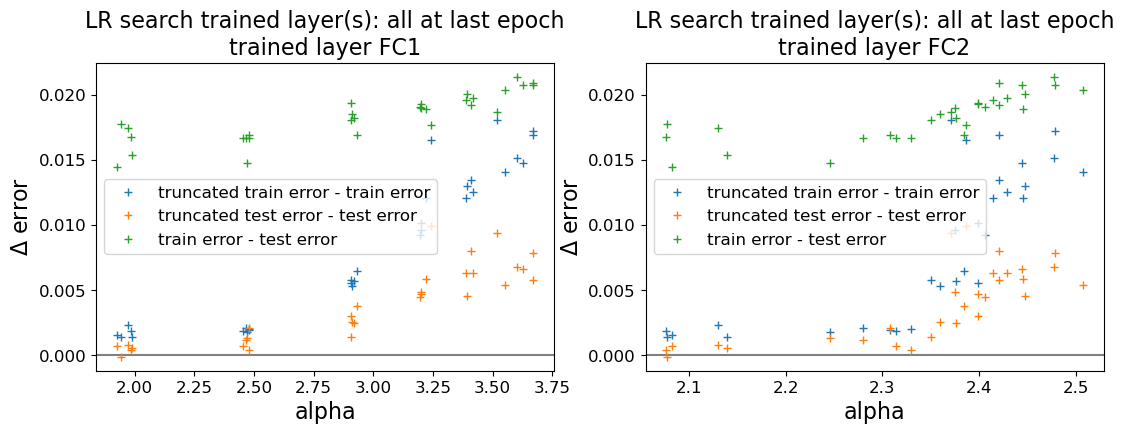
\includegraphics[width=12cm]{img/truncated_error/mlp3_trunc_error_by_LR_alpha_all_xmin.png}
  \caption{
        Train and test error gaps using the \POWERLAW~MSR, as a function of alpha in the FC1 and FC2 layers of MLP3 
        models, at the \emph{final epoch} of training. We can see that as alpha decreases towards $2$, (right to left), 
        $\Delta E_{train}$ and $\Delta E_{test}$ generally decrease as well, meaning that the closer $\ALPHA$ is to $2$, 
        the more the Effective Correllation Space explains the train and test predictions. The gap between un-truncated 
        train and test error, (\EQN \ref{eqn:gen_gap},) generally decreases as well until $\alpha_{FC1} < 2$.
  }
  \label{fig:mlp3-alpha-generalization-gap}
\end{figure}

In both layers, $\Delta E_{train}$ and $\Delta E_{test}$ steadily decrease with $\alpha_{FC1}$, until it passes below 
$2$, after which the relation deteriorates somewhat.
This is especially prominent in FC2. 
Recall from Figure~\ref{fig:mlp3-alphas-lr}, Section~\ref{sxn:empirical-test_acc}, that when $\alpha_{FC1}$ passed below $2$, the train error and test error both increased and exhibited larger variability. 
From this we interpret \ALPHA as a measure of \emph{regularization} (which is consistent with its introduction as a measure of 
implicit self-regularization~\cite{MM18_TR_JMLRversion}).
Regularization has the effect of keeping train and test accuracy closer together, and generally, as \ALPHA in the dominant layer decreases towards $2$ from above, the train-test error gap decreases.


